%==================================
%          Introduction
%==================================
\section{\review{Introduction}}


%----------------------------------
%           Motivation
%----------------------------------
\subsection{\review{Motivation}}

Beam-based measurements have been carried in the LHC since Run 1 to better understand the decapolar
fields. Those have been carried out via chromaticity
measurements~\cite{maclean_non-linear_2011,maclean_commissioning_2016,maclean_measurement_2014}. 
The third order of the non-linear chromaticity, $Q'''$, generated for the most part by decapoles,
has shown a consistent discrepancy at injection energy between its expected value from simulations
and that observed. \Cref{fig:decapoles:bare_chroma_vs_simulations} highlights this
discrepancy.

\begin{figure}[!htb]
    \centering
    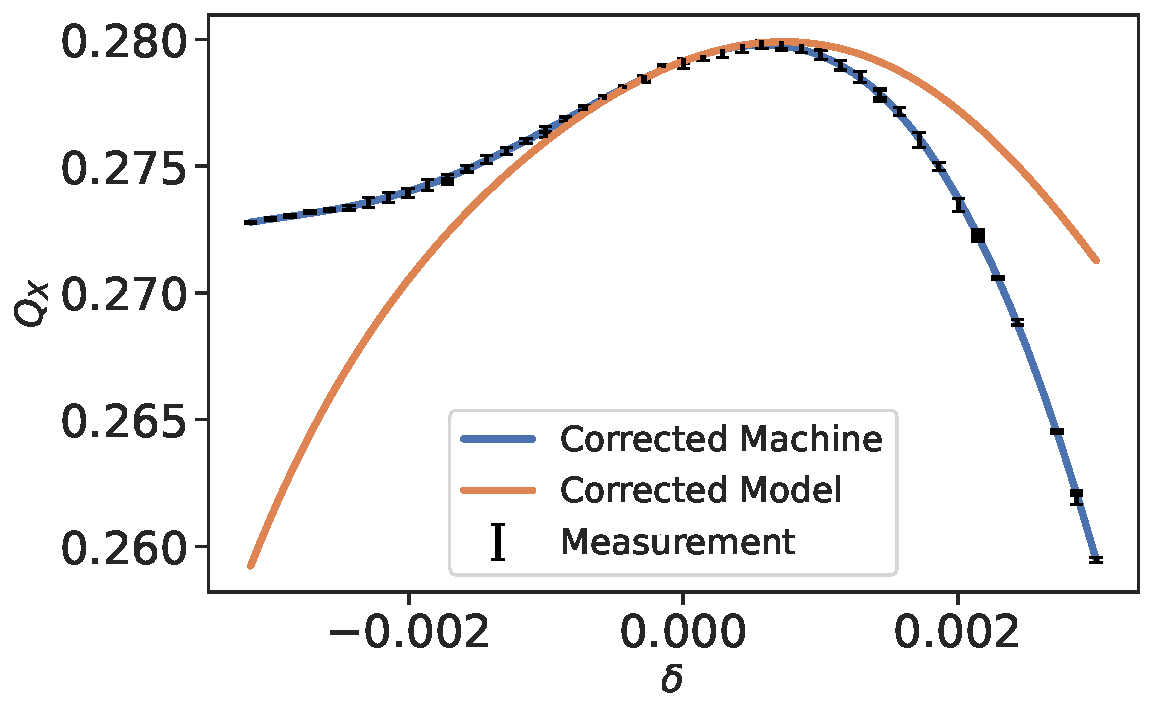
\includegraphics[width=0.8\textwidth]{images/dq3_corrected_simulation_fidel.pdf}
    \caption{Measured and simulated chromaticity with application of the nominal decapolar
    corrections from FiDeL. It can be seen that although the corrections should diminish $Q'''$, it
    is not well corrected in practice.}
    \label{fig:decapoles:bare_chroma_vs_simulations}
\end{figure}

The FiDeL model, based on magnetic measurements, is used during operation to correct various
multipole errors, including octupolar and decapolar. The operational corrections being based on this
magnetic model and simulations, the residual $Q'''$ value is expected to be small, which is however
not the case.  Chromaticity measurements have thus been repeated during LHC's Run 3 and corrections
made routine, aimed at correcting the observed discrepancy.

The study of non-linear chromaticity has proven valuable in quantifying decapolar fields, yet it
does not permit alone to understand the exact origins of the observed discrepancy. In an effort to
gain deeper insights, additional measurements were performed focusing on novel observables that had
not been previously explored.
\textit{Bare chromaticity} involves measuring chromaticity with
the octupolar an decapolar correctors deactivated ; this approach aims to isolate the machine
effects from those of the correctors.
\textit{Chromatic amplitude detuning}, evaluates how the tune varies with both the beam's action and
the momentum offset ; this methods has the benefit of having a different expression that of the
chromaticity.

Complementing those measurements, studies of decapolar Resonance Driving Terms have been undertaken
for the first time in the LHC. Contributing to resonances close to the working, those RDTs also have
benefited from corrections.


%----------------------------------
%       Decapolar Correctors
%----------------------------------
\subsection{\review{Decapolar Correctors}}

As seen in \cref{fig:introduction:lhc_arc_cell}, the LHC is equipped with decapoles. Those magnets
are part of the LHC's design report, aiming at correcting the field errors of the main dipoles.
Those correctors, denominated \textit{MCD}, are specific to each beam and are placed after every
second dipole, totaling 1232 in number~\cite{venturini_delsolaro_magnetic_2005}.
MCDs are nested with octupolar correctors, \textit{MCO}. The pair of those correctors of often
referred to as \textit{MCDO}. 
It is not possible to individually power each corrector. Rather, a circuit consists of a whole arc.
There are in total 16 circuits to control the correctors of both beams and 8 arcs.
\Cref{fig:decapoles:decapole_picture} shows a picture taken of decapoles on a test bench.

\begin{figure}
    \centering
    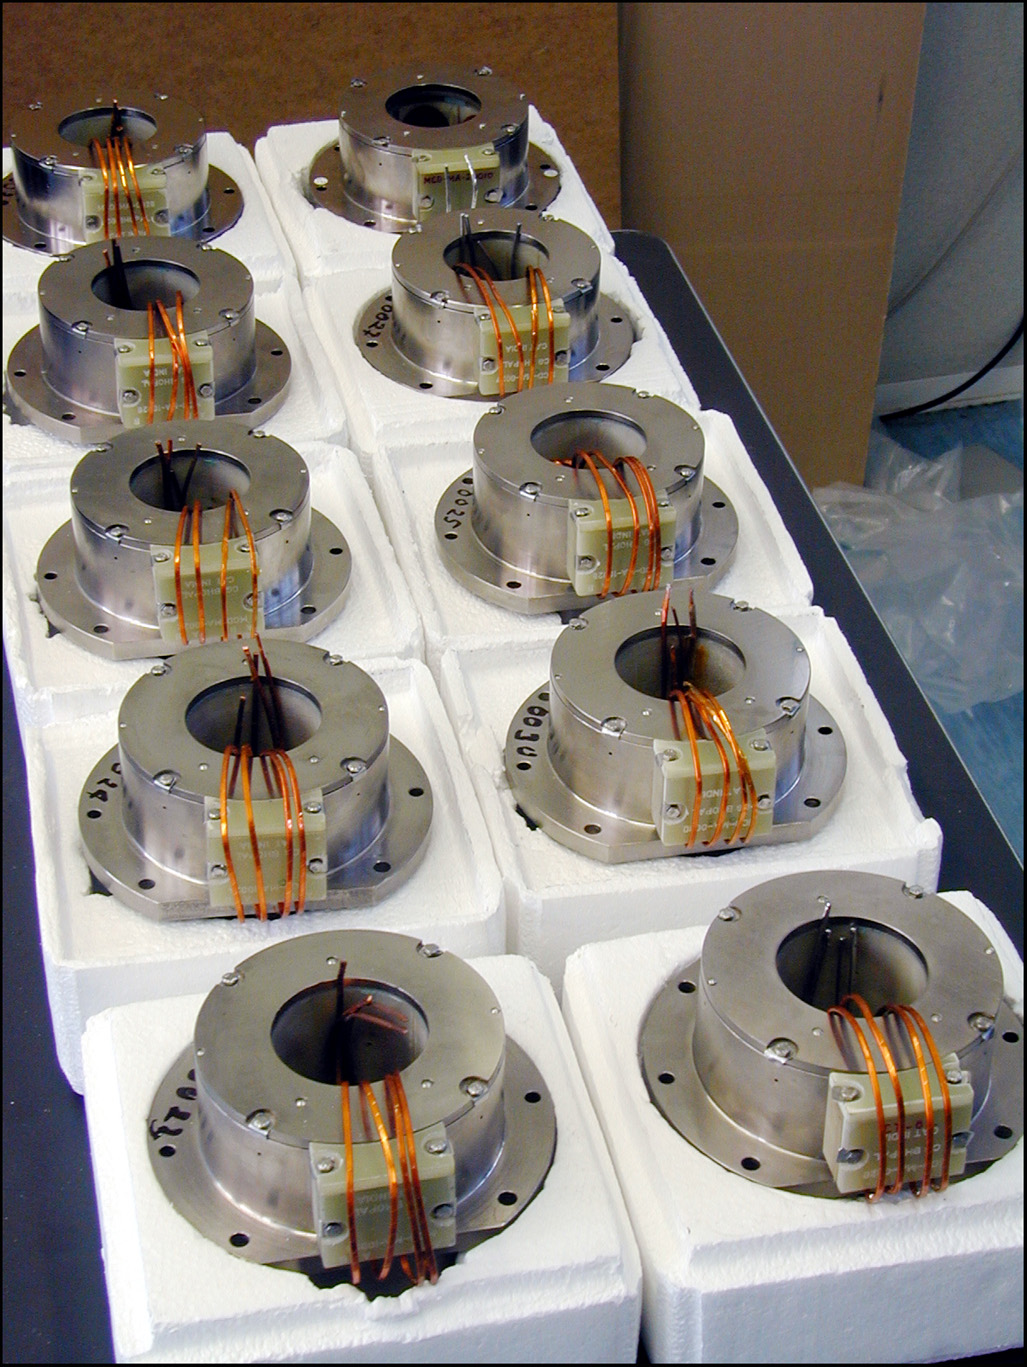
\includegraphics[width=0.4\textwidth]{./images/decapoles_real_pic.jpg}
    \caption{Decapoles on a test bench, being inspected after
    manufacturing~\cite{noauthor_ten_2001}.}
    \label{fig:decapoles:decapole_picture}
\end{figure}


The important characteristics of the magnetic fields of correctors are their main field transfer
function (or \textit{response}), the field quality and possible crosstalk, as MCOs and MCDs are
nested~\cite{venturini_delsolaro_magnetic_2005}.
In order to determine the aforementioned discrepancy, the decapole correctors themselves need to be
studied, to rule any possible unwanted effects.


% -------- Strengths at Injection
\paragraph{Strengths at Injection}

%\begin{wraptable}{r}{0.4\textwidth}
\begin{table}
    \centering
    \begin{tabular}{lr}
        \toprule
        Circuit   & $K_5 [\textrm{m}^{-5}]$ \\
        \midrule
        Beam 1    & \\
        \hspace{2mm}RCD.A12B1 & $-4582$ \\
        \hspace{2mm}RCD.A23B1 & $-5106$ \\
        \hspace{2mm}RCD.A34B1 & $-4855$ \\
        \hspace{2mm}RCD.A45B1 & $-4577$ \\
        \hspace{2mm}RCD.A56B1 & $-4125$ \\
        \hspace{2mm}RCD.A67B1 & $-5166$ \\
        \hspace{2mm}RCD.A78B1 & $-6827$ \\
        \hspace{2mm}RCD.A81B1 & $-5500$ \\
        Beam 2    & \\
        \hspace{2mm}RCD.A12B2 & $-4490$ \\
        \hspace{2mm}RCD.A23B2 & $-5155$ \\
        \hspace{2mm}RCD.A34B2 & $-4825$ \\
        \hspace{2mm}RCD.A45B2 & $-4619$ \\
        \hspace{2mm}RCD.A56B2 & $-4064$ \\
        \hspace{2mm}RCD.A67B2 & $-5066$ \\
        \hspace{2mm}RCD.A78B2 & $-6866$ \\
        \hspace{2mm}RCD.A81B2 & $-5446$ \\
        \bottomrule
    \end{tabular}
    \caption{Strength of decapolar correctors at injection energy for FiDeL corrections.}
    \label{tab:decapoles:strength_rcd_fidel}
%\end{wraptable}
\end{table}

At injection energy, the decapoles are powered to a static strength. New optics introduced
throughout the years often have for effect to vary slightly the $\beta$-function along the ring,
having thus an impact on the chromaticity, as seen in
\cref{eq:detuning_effects:chromaticity_strength}. New corrections are then computed via FiDeL to
account for it.
Although those corrections vary throughout the years, the shift is in practice fairly negligible.
\Cref{tab:decapoles:rdts:correction_f1004_k5}, a bit further in this chapter, shows the strength of
the correctors and the related circuits at injection energy for the optics deployed in 2024.